\renewcommand{\FileName}{corresp}
\subsection{Basic ideas}
\begin{frame}[squeeze]
  \frametitle{Correspondence analysis}
  \begin{block}{\large\bfseries Correspondence analysis (CA)} 
     Analog of PCA for frequency data: 
      \begin{itemize*}
	  \item account for maximum \% of $\chi^2$ in few (2-3) dimensions
	  \item finds scores for row ($x_{im}$) and column ($y_{jm}$) categories on these dimensions
	  \item uses Singular Value Decomposition of residuals from independence,
	  $d_{ij} = (n_{ij} - \widehat{m}_{ij}) / \sqrt{\widehat{m}_{ij}}$
\begin{equation*}
  \frac{  d_{ij}} { \sqrt { n } }
 = \sum_{m=1}^M  \lambda_m \,  x_{im} \,  y_{jm}
\end{equation*}
	  \item \emph{optimal scaling}:  each pair of scores for rows ($x_{im}$) and columns ($y_{jm}$) have highest
	  possible correlation ($= \lambda_m$).
	  \item plots of the row ($x_{im}$) and column ($y_{jm}$) scores show associations
	  \end{itemize*}
  \end{block}
\end{frame}


\begin{frame}
Hair color, Eye color data:
 \begin{center}
  \includegraphics[height=.72\textheight,clip]{fig/corresp2a}
  \begin{itemize*}
  \item Interpretation:  row/column points ``near'' each other are positively associated
  \item Dim 1: 89.4\% of $\chi^2$ (dark $\leftrightarrow$ light)
  \item Dim 2: 9.5\% of $\chi^2$ (RED/Green vs.\ others)
  \end{itemize*}
 \end{center}
\end{frame}

\begin{frame}[fragile]
  \frametitle{\PROC{CORRESP} and the \macrot{CORRESP}}
  \begin{itemize}
	\item Two forms of input \Dset:
      \begin{itemize*}
	  \item \Dset\ in \emph{contingency table} form -- column variables are levels of one factor,
	  observations (rows) are levels of the other.
\begin{listing}[frame=single,baselinestretch=0.9]
Obs     Eye     BLACK    BROWN    RED    BLOND

 1     Brown      68      119      26       7 
 2     Blue       20       84      17      94 
 3     Hazel      15       54      14      10 
 4     Green       5       29      14      16 
\end{listing}

	  \item Raw category responses (\emph{case form}), or cell frequencies (\emph{frequency form}),
	  classified by 2 or more factors (e.g., output from \PROC{FREQ})
\begin{listing}[frame=single,baselinestretch=0.9]
Obs     Eye     HAIR      Count

  1    Brown    BLACK       68
  2    Brown    BROWN      119
  3    Brown    RED         26
  4    Brown    BLOND        7
  ...
 15    Green    RED         14
 16    Green    BLOND       16
\end{listing}
	  \end{itemize*}
  \end{itemize}

\end{frame}

\begin{frame}
  \frametitle{Software: \PROC{CORRESP}, \macrot{CORRESP} \& R}
  \begin{itemize}
	\item<-1>{\large\bfseries \PROC{CORRESP}}
      \begin{itemize*}
	  \item Handles 2-way CA, extensions to \nway\ tables, and MCA
	  \item Many options for scaling row/column coordinates and output statistics
	  \item \texttt{OUTC=} option $\rightarrow$ \ODS\ for plotting
	  \item  SAS V9.1+: \PROC{CORRESP} uses ODS Graphics
      \end{itemize*}
	  
	\item<2->{\large\bfseries \macro{CORRESP}}
      \begin{itemize*}
	  \item Uses \PROC{CORRESP} for analysis
	  \item Produces labeled plots of the category points in either 2 or 3 dimensions
	  \item Many graphic options; can equate axes automatically
	  \item See: \url{http://datavis.ca/sasmac/corresp.html}
      \end{itemize*}

	\item<3->{\large\bfseries \proglang{R}}
      \begin{itemize*}
     \item The \pkg{ca} provides 2-way CA, MCA and more
	 \item \texttt{plot(ca(data))} gives reasonable (but not yet beautiful) plots
	 \item Other R packages: caGUI, vegan, ade4, FactoMiner, ...
      \end{itemize*}
 \end{itemize}

\end{frame}

\begin{frame}[fragile]
  \frametitle{Example: Hair and Eye Color}
  \begin{itemize}
	\item {\large\bfseries Input the data} in contingency table form

\vspace{2ex}
\begin{Input}[label=\fbox{\texttt{corresp2a.sas} $\cdots$},baselinestretch=0.9]
data haireye;
  input  EYE $ BLACK BROWN RED BLOND ; \ignore{$}
  datalines;
        Brown    68   119    26     7    
        Blue     20    84    17    94    
        Hazel    15    54    14    10    
        Green     5    29    14    16    
;
\end{Input}
  \end{itemize}
\end{frame}

\begin{frame}[fragile]
  \frametitle{Example: Hair and Eye Color}

  \begin{itemize}
	\item{\large\bfseries Using \PROC{CORRESP} directly}--- ODS graphics (V9.1+)
\begin{Input}[baselinestretch=0.9,numbers=none]
ods rtf; \sascomment{/* ODS destination: rtf, html, latex, ... */}
\sasemph{ods graphics on;}
proc corresp data=haireye short;
  id eye;                         \sascomment{/* row variable  */}
  var black brown red blond;      \sascomment{/* col variables */}
\sasemph{ods graphics off;}
ods rtf close;
\end{Input}
	\item{\large\bfseries Using the \macro{CORRESP}}--- labeled high-res plot
\begin{Input}[baselinestretch=0.9,numbers=none]
%corresp (data=haireye, 
    id=eye,                     \sascomment{/* row variable  */}
    var=black brown red blond,  \sascomment{/* col variables */}
    dimlab=Dim);                \sascomment{/* options       */}
\end{Input}
  \end{itemize}
\end{frame}

\begin{frame}[fragile]
  \frametitle{Example: Hair and Eye Color}
Printed output:
\begin{Output}[fontsize=\footnotesize,baselinestretch=0.7,gobble=5]
                    The Correspondence Analysis Procedure

                     Inertia and Chi-Square Decomposition

       Singular  Principal Chi-
       Values    Inertias  Squares Percents   18   36   54   72   90
                                           ----+----+----+----+----+---
       0.45692   0.20877   123.593  89.37% *************************
       0.14909   0.02223    13.158   9.51% ***
       0.05097   0.00260     1.538   1.11%
                 -------   -------
                 0.23360    138.29 (Degrees of Freedom = 9)

                               Row Coordinates
                                     Dim1          Dim2

                      Brown      -.492158      -.088322
                      Blue       0.547414      -.082954
                      Hazel      -.212597      0.167391
                      Green      0.161753      0.339040

                              Column Coordinates
                                     Dim1          Dim2

                      BLACK      -.504562      -.214820
                      BROWN      -.148253      0.032666
                      RED        -.129523      0.319642
                      BLOND      0.835348      -.069579
\end{Output}
\end{frame}

\begin{frame}[fragile]
  \frametitle{Example: Hair and Eye Color}
Output \Dset (selected variables):
\begin{Output}[fontsize=\footnotesize,baselinestretch=0.8,gobble=3]
     Obs    _TYPE_      EYE       DIM1        DIM2

      1     INERTIA               .           .
      2     OBS        Brown    -0.49216    -0.08832
      3     OBS        Blue      0.54741    -0.08295
      4     OBS        Hazel    -0.21260     0.16739
      5     OBS        Green     0.16175     0.33904
      6     VAR        BLACK    -0.50456    -0.21482
      7     VAR        BROWN    -0.14825     0.03267
      8     VAR        RED      -0.12952     0.31964
      9     VAR        BLOND     0.83535    -0.06958
\end{Output}
Row and column points are distinguished by the \verb|_TYPE_| variable: \texttt{OBS} vs.\ \texttt{VAR}
\end{frame}

\begin{frame}
  \frametitle{Example: Hair and Eye Color}
Graphic output from \macro{CORRESP}:
 \begin{center}
  \includegraphics[height=.72\textheight,clip]{fig/corresp2a}
%   \begin{itemize*}
%   \item Top legend produced with Annotate data set and the \texttt{INANNO=} option to the \macro{CORRESP}
%   \end{itemize*}
 \end{center}
\end{frame}

\subsection{CA in R}
\renewcommand{\FileName}{ca-R}

\begin{frame}[fragile]
	\frametitle{CA in R: the \pkg{ca}}

\begin{Rin}[baselinestretch=0.8,fontsize=\footnotesize]
> HairEye <- margin.table(HairEyeColor, c(1, 2))
> library(ca)
> ca(HairEye)
\end{Rin}
%Printed output:
\begin{Rout}[baselinestretch=0.8,fontsize=\footnotesize]
 Principal inertias (eigenvalues):
           1        2        3       
Value      0.208773 0.022227 0.002598
Percentage 89.37%   9.52%    1.11%   
 ...
\end{Rout}
Plot the \texttt{ca} object:
\begin{Rin}
> plot(ca(HairEye), main="Hair Color and Eye Color")
\end{Rin}

\begin{center}
\includegraphics[height=.46\textheight,trim=5 20 5 10]{fig/ca-haireye}
\end{center}
\end{frame}

\subsection{Multi-way tables}
\begin{frame}
  \frametitle{Multi-way tables}
Correspondence analysis can be extended to $n$-way tables in several ways:
  \begin{itemize}
	\item<1-> {\large\bfseries Multiple correspondence analysis (MCA)} 
		\begin{itemize*}
     	  \item Extends CA to $n$-way tables
          \item only uses bivariate associations 
		\end{itemize*}

    \item<2-> {\large\bfseries Stacking approach}
 		\begin{itemize*}
         \item $n$-way table flattened to a 2-way table, combining several variables ``interactively''
		 \item Each way of stacking corresponds to a \emph{\loglin\ model}
         \item Ordinary CA of the flattened table $\rightarrow$ visualization of that model
         \item Associations among stacked variables are \emph{not visualized}
		\end{itemize*}
	\item<3-> Here, I only describe the stacking approach, and only with SAS
		\begin{itemize*}
		\item In SAS 9.3, the \texttt{MCA} option with \PROC{CORRESP} provides some reasonable plots.
		 \item For R, see the \pkg{ca}-- the \func{mjca} function is much more general
		\end{itemize*}

   \end{itemize}
\end{frame}

\begin{frame}<none>
  \frametitle{Multi-way tables}
  \begin{itemize}
	\item{\large\bfseries Stacking approach:} \citet{HeijdenLeeuw:85}--- 
      \begin{itemize*}
	  \item three-way table, of size \(I \times  J \times  K\) can be sliced and stacked as
	a two-way table, of size \((I \times  J ) \times  K\)
 \begin{center}
  \includegraphics[height=.45\textheight,clip]{fig/stacking}
 \end{center}

	  \item The variables combined are treated ``interactively''
	  \item Each way of stacking corresponds to a \loglin\ model
    	\begin{itemize*}
		\item \((I \times  J ) \times  K\) $\rightarrow$ [AB][C]
		\item \(I \times  ( J \times  K )\) $\rightarrow$ [A][BC]
		\item \(J \times  ( I \times  K )\) $\rightarrow$ [B][AC]
		\end{itemize*}
	  \item Only the associations in separate [] terms are analyzed and displayed
	  \end{itemize*}
  \end{itemize}
\end{frame}

\begin{frame}
  \frametitle{Multi-way tables: Stacking}
  \begin{itemize}
	\item{\large\bfseries Stacking approach:} \citet{HeijdenLeeuw:85}--- 
      \begin{itemize*}
	  \item three-way table, of size \(I \times  J \times  K\) can be sliced and stacked as
	a two-way table, of size \((I \times  J ) \times  K\)
 	  \end{itemize*}
 \end{itemize}

 \begin{minipage}[c]{.49\linewidth}
  \includegraphics[width=1\linewidth,clip]{fig/stacking}
 \end{minipage}%
 \hfill
 \begin{minipage}[c]{.49\linewidth}
       \begin{itemize*}
	  \item The variables combined are treated ``interactively''
	  \item Each way of stacking corresponds to a \loglin\ model
    	\begin{itemize*}
		\item \((I \times  J ) \times  K\) $\rightarrow$ [AB][C]
		\item \(I \times  ( J \times  K )\) $\rightarrow$ [A][BC]
		\item \(J \times  ( I \times  K )\) $\rightarrow$ [B][AC]
		\end{itemize*}
	  \item Only the associations in separate [] terms are analyzed and displayed
	  \end{itemize*}
\end{minipage}
\end{frame}

\begin{frame}[fragile]
  \frametitle{Multi-way tables: Stacking}
  \begin{itemize}
	\item{\large\bfseries \PROC{CORRESP}}:  Use \texttt{TABLES} statement and option
	\texttt{CROSS=ROW} or \texttt{CROSS=COL}.  E.g., for model [A B] [C],
\begin{listing}
proc corresp cross=row;
   tables A B, C;
   weight count;
\end{listing}

	\item{\large\bfseries \macro{CORRESP}}: Can use \verb|/| instead of \verb|,|
\begin{listing}
%corresp(
   options=cross=row,
   tables=A B/ C,
   weight count);
\end{listing}
  \end{itemize}

\end{frame}

\begin{frame}[fragile]
  \frametitle{Example: Suicide Rates}
Suicide rates in West Germany, by Age, Sex and Method of suicide
\begin{Output}[baselinestretch=0.9]
   Sex  Age    POISON     GAS    HANG   DROWN     GUN    JUMP

    M  10-20     1160     335    1524      67     512     189
    M  25-35     2823     883    2751     213     852     366
    M  40-50     2465     625    3936     247     875     244
    M  55-65     1531     201    3581     207     477     273
    M  70-90      938      45    2948     212     229     268

    F  10-20      921      40     212      30      25     131
    F  25-35     1672     113     575     139      64     276
    F  40-50     2224      91    1481     354      52     327
    F  55-65     2283      45    2014     679      29     388
    F  70-90     1548      29    1355     501       3     383
\end{Output}
  \begin{itemize}
	\item CA of the [Age Sex] by [Method] table:
      \begin{itemize*}
	  \item Shows associations between the Age-Sex combinations and Method
	  \item Ignores association between Age and Sex
	  \end{itemize*}
  \end{itemize}
\end{frame}

\begin{frame}[fragile]
  \frametitle{Example: Suicide Rates}
\vspace{2ex}
\begin{Input}[label=\fbox{\texttt{suicide5.sas} $\cdots$},baselinestretch=0.9]
%include catdata(suicide);
   \sascomment{*-- equate axes!;}
axis1 order=(-.7 to .7 by .7) length=6.5 in label=(a=90 r=0);
axis2 order=(-.7 to .7 by .7) length=6.5 in;
%corresp(data=suicide,  weight=count,
    \sasemph{tables=%str(age sex, method)}, 
    \sasemph{options=cross=row} short, 
    vaxis=axis1, haxis=axis2);
\end{Input}
Output:
\begin{Output}[fontsize=\footnotesize,baselinestretch=0.8]
                   Inertia and Chi-Square Decomposition

     Singular  Principal Chi-
     Values    Inertias  Squares Percents   12   24   36   48   60
                                         ----+----+----+----+----+---
     0.32138   0.10328   5056.91  60.41% *************************
     0.23736   0.05634   2758.41  32.95% **************
     0.09378   0.00879    430.55   5.14% **
     0.04171   0.00174     85.17   1.02%
     0.02867   0.00082     40.24   0.48%
               -------   -------
               0.17098   8371.28 (Degrees of Freedom = 45)
\end{Output}
\end{frame}

\begin{frame}
CA Graph:
 \begin{center}
  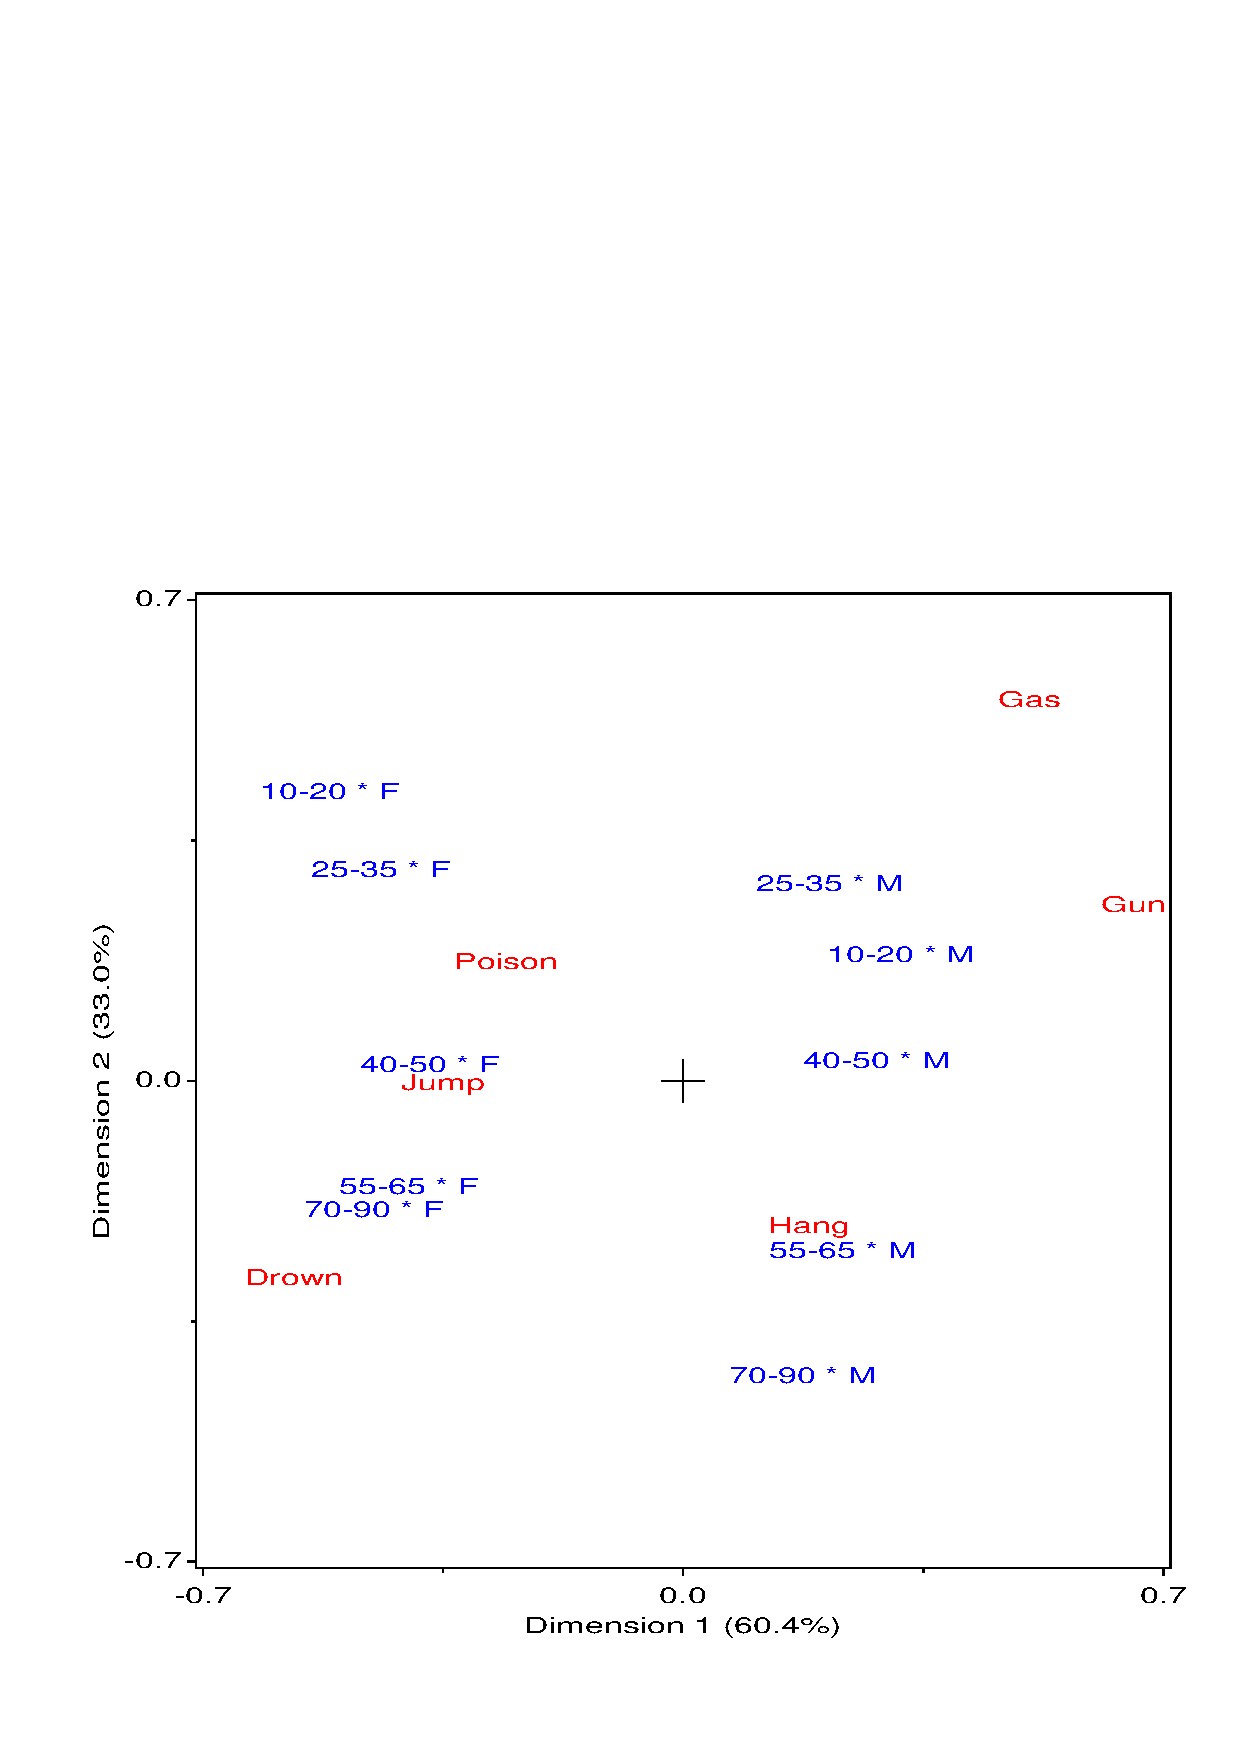
\includegraphics[height=.9\textheight,clip]{fig/suicide51}
 \end{center}
\end{frame}

\begin{frame}
Looking forward--- View this as a mosaic display:
 \begin{center}
  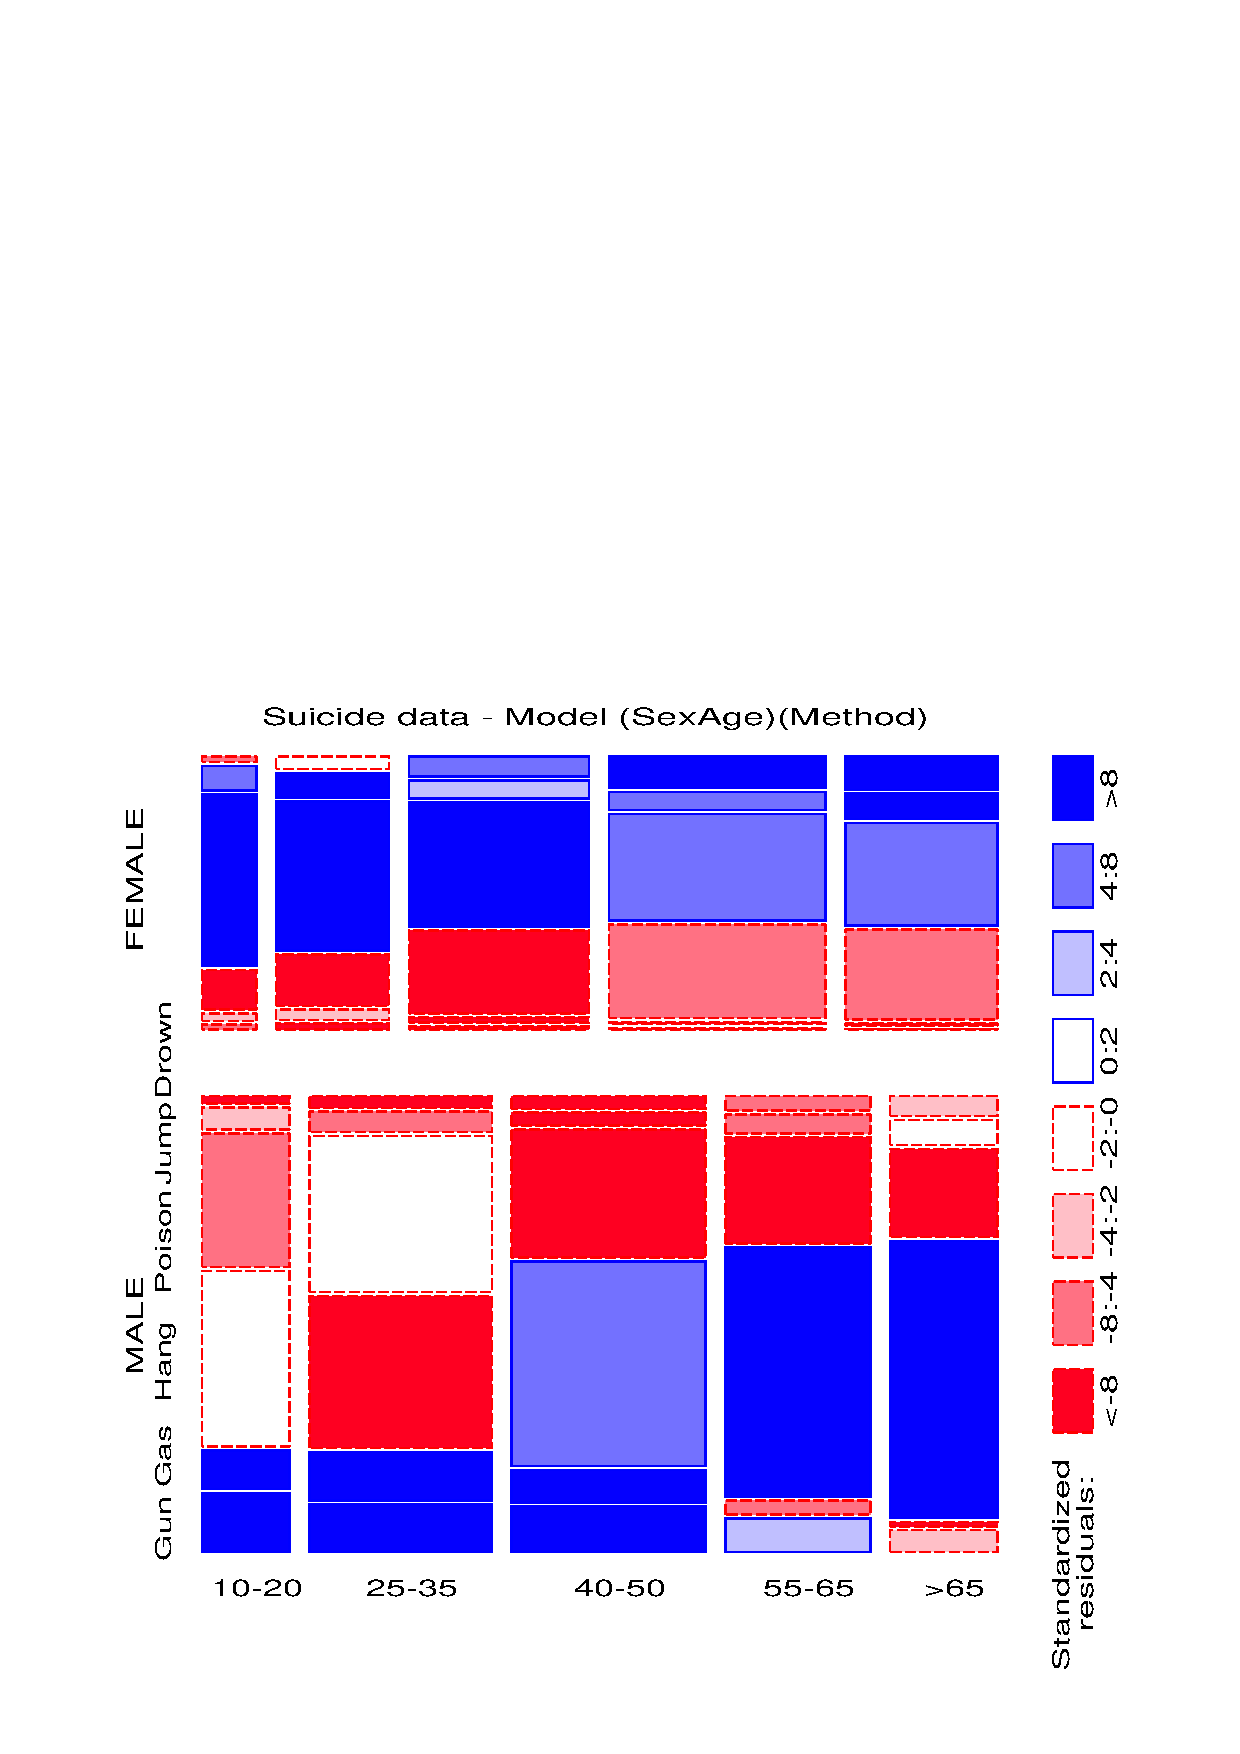
\includegraphics[height=.9\textheight,clip]{fig/mosaic6b}
 \end{center}
\end{frame}

\endinput
% slide template
\begin{frame}
  \frametitle{}
  \begin{itemize}
	\item{\large\bfseries }
      \begin{itemize*}
	  \item 
    	\begin{itemize*}
		\item 
		\item 
		\end{itemize*}
	  \item 
	  \end{itemize*}
	\item{\large\bfseries }
	\item{\large\bfseries }
  \end{itemize}
\end{frame}

